% Options for packages loaded elsewhere
\PassOptionsToPackage{unicode}{hyperref}
\PassOptionsToPackage{hyphens}{url}
%
\documentclass[
]{book}
\usepackage{amsmath,amssymb}
\usepackage{lmodern}
\usepackage{iftex}
\ifPDFTeX
  \usepackage[T1]{fontenc}
  \usepackage[utf8]{inputenc}
  \usepackage{textcomp} % provide euro and other symbols
\else % if luatex or xetex
  \usepackage{unicode-math}
  \defaultfontfeatures{Scale=MatchLowercase}
  \defaultfontfeatures[\rmfamily]{Ligatures=TeX,Scale=1}
\fi
% Use upquote if available, for straight quotes in verbatim environments
\IfFileExists{upquote.sty}{\usepackage{upquote}}{}
\IfFileExists{microtype.sty}{% use microtype if available
  \usepackage[]{microtype}
  \UseMicrotypeSet[protrusion]{basicmath} % disable protrusion for tt fonts
}{}
\makeatletter
\@ifundefined{KOMAClassName}{% if non-KOMA class
  \IfFileExists{parskip.sty}{%
    \usepackage{parskip}
  }{% else
    \setlength{\parindent}{0pt}
    \setlength{\parskip}{6pt plus 2pt minus 1pt}}
}{% if KOMA class
  \KOMAoptions{parskip=half}}
\makeatother
\usepackage{xcolor}
\IfFileExists{xurl.sty}{\usepackage{xurl}}{} % add URL line breaks if available
\IfFileExists{bookmark.sty}{\usepackage{bookmark}}{\usepackage{hyperref}}
\hypersetup{
  pdftitle={Notas de Clase: Series de Tiempo},
  pdfauthor={Benjamín Oliva, Omar Alfaro-Rivera y Emiliano Pérez Caullieres},
  hidelinks,
  pdfcreator={LaTeX via pandoc}}
\urlstyle{same} % disable monospaced font for URLs
\usepackage{color}
\usepackage{fancyvrb}
\newcommand{\VerbBar}{|}
\newcommand{\VERB}{\Verb[commandchars=\\\{\}]}
\DefineVerbatimEnvironment{Highlighting}{Verbatim}{commandchars=\\\{\}}
% Add ',fontsize=\small' for more characters per line
\usepackage{framed}
\definecolor{shadecolor}{RGB}{248,248,248}
\newenvironment{Shaded}{\begin{snugshade}}{\end{snugshade}}
\newcommand{\AlertTok}[1]{\textcolor[rgb]{0.94,0.16,0.16}{#1}}
\newcommand{\AnnotationTok}[1]{\textcolor[rgb]{0.56,0.35,0.01}{\textbf{\textit{#1}}}}
\newcommand{\AttributeTok}[1]{\textcolor[rgb]{0.77,0.63,0.00}{#1}}
\newcommand{\BaseNTok}[1]{\textcolor[rgb]{0.00,0.00,0.81}{#1}}
\newcommand{\BuiltInTok}[1]{#1}
\newcommand{\CharTok}[1]{\textcolor[rgb]{0.31,0.60,0.02}{#1}}
\newcommand{\CommentTok}[1]{\textcolor[rgb]{0.56,0.35,0.01}{\textit{#1}}}
\newcommand{\CommentVarTok}[1]{\textcolor[rgb]{0.56,0.35,0.01}{\textbf{\textit{#1}}}}
\newcommand{\ConstantTok}[1]{\textcolor[rgb]{0.00,0.00,0.00}{#1}}
\newcommand{\ControlFlowTok}[1]{\textcolor[rgb]{0.13,0.29,0.53}{\textbf{#1}}}
\newcommand{\DataTypeTok}[1]{\textcolor[rgb]{0.13,0.29,0.53}{#1}}
\newcommand{\DecValTok}[1]{\textcolor[rgb]{0.00,0.00,0.81}{#1}}
\newcommand{\DocumentationTok}[1]{\textcolor[rgb]{0.56,0.35,0.01}{\textbf{\textit{#1}}}}
\newcommand{\ErrorTok}[1]{\textcolor[rgb]{0.64,0.00,0.00}{\textbf{#1}}}
\newcommand{\ExtensionTok}[1]{#1}
\newcommand{\FloatTok}[1]{\textcolor[rgb]{0.00,0.00,0.81}{#1}}
\newcommand{\FunctionTok}[1]{\textcolor[rgb]{0.00,0.00,0.00}{#1}}
\newcommand{\ImportTok}[1]{#1}
\newcommand{\InformationTok}[1]{\textcolor[rgb]{0.56,0.35,0.01}{\textbf{\textit{#1}}}}
\newcommand{\KeywordTok}[1]{\textcolor[rgb]{0.13,0.29,0.53}{\textbf{#1}}}
\newcommand{\NormalTok}[1]{#1}
\newcommand{\OperatorTok}[1]{\textcolor[rgb]{0.81,0.36,0.00}{\textbf{#1}}}
\newcommand{\OtherTok}[1]{\textcolor[rgb]{0.56,0.35,0.01}{#1}}
\newcommand{\PreprocessorTok}[1]{\textcolor[rgb]{0.56,0.35,0.01}{\textit{#1}}}
\newcommand{\RegionMarkerTok}[1]{#1}
\newcommand{\SpecialCharTok}[1]{\textcolor[rgb]{0.00,0.00,0.00}{#1}}
\newcommand{\SpecialStringTok}[1]{\textcolor[rgb]{0.31,0.60,0.02}{#1}}
\newcommand{\StringTok}[1]{\textcolor[rgb]{0.31,0.60,0.02}{#1}}
\newcommand{\VariableTok}[1]{\textcolor[rgb]{0.00,0.00,0.00}{#1}}
\newcommand{\VerbatimStringTok}[1]{\textcolor[rgb]{0.31,0.60,0.02}{#1}}
\newcommand{\WarningTok}[1]{\textcolor[rgb]{0.56,0.35,0.01}{\textbf{\textit{#1}}}}
\usepackage{longtable,booktabs,array}
\usepackage{calc} % for calculating minipage widths
% Correct order of tables after \paragraph or \subparagraph
\usepackage{etoolbox}
\makeatletter
\patchcmd\longtable{\par}{\if@noskipsec\mbox{}\fi\par}{}{}
\makeatother
% Allow footnotes in longtable head/foot
\IfFileExists{footnotehyper.sty}{\usepackage{footnotehyper}}{\usepackage{footnote}}
\makesavenoteenv{longtable}
\usepackage{graphicx}
\makeatletter
\def\maxwidth{\ifdim\Gin@nat@width>\linewidth\linewidth\else\Gin@nat@width\fi}
\def\maxheight{\ifdim\Gin@nat@height>\textheight\textheight\else\Gin@nat@height\fi}
\makeatother
% Scale images if necessary, so that they will not overflow the page
% margins by default, and it is still possible to overwrite the defaults
% using explicit options in \includegraphics[width, height, ...]{}
\setkeys{Gin}{width=\maxwidth,height=\maxheight,keepaspectratio}
% Set default figure placement to htbp
\makeatletter
\def\fps@figure{htbp}
\makeatother
\setlength{\emergencystretch}{3em} % prevent overfull lines
\providecommand{\tightlist}{%
  \setlength{\itemsep}{0pt}\setlength{\parskip}{0pt}}
\setcounter{secnumdepth}{5}
\usepackage{booktabs}
\ifLuaTeX
  \usepackage{selnolig}  % disable illegal ligatures
\fi
\usepackage[]{natbib}
\bibliographystyle{apalike}

\title{Notas de Clase: Series de Tiempo}
\author{Benjamín Oliva, Omar Alfaro-Rivera y Emiliano Pérez Caullieres}
\date{2022-07-11}

\usepackage{amsthm}
\newtheorem{theorem}{Theorem}[chapter]
\newtheorem{lemma}{Lemma}[chapter]
\newtheorem{corollary}{Corollary}[chapter]
\newtheorem{proposition}{Proposition}[chapter]
\newtheorem{conjecture}{Conjecture}[chapter]
\theoremstyle{definition}
\newtheorem{definition}{Definition}[chapter]
\theoremstyle{definition}
\newtheorem{example}{Example}[chapter]
\theoremstyle{definition}
\newtheorem{exercise}{Exercise}[chapter]
\theoremstyle{definition}
\newtheorem{hypothesis}{Hypothesis}[chapter]
\theoremstyle{remark}
\newtheorem*{remark}{Remark}
\newtheorem*{solution}{Solution}
\begin{document}
\maketitle

{
\setcounter{tocdepth}{1}
\tableofcontents
}
\hypertarget{introducciuxf3n}{%
\chapter{Introducción}\label{introducciuxf3n}}

Estas notas son un resumen, una síntesis comparativa y, en algunos casos, una interpretación propia de los libros de texto de Cowpertwait y Metcalfe (2009), Guerrero-Guzman (2014), Enders (2015), Franses y van Dijk (2003), Kirchgassner, Wolters, y Hassler (2012), Lutkepohl (2005), Wei (2019), entre
otros. En algunos casos se incorpora información adicional para efectos de dar contexto al tema analizado (ver sección de Bibliografía para mayores detalles).

El objetivo de este documento es proporcionar un conjunto de apuntes que sirva de apoyo para la clase, por ello no deben considerarse como notas exhaustivas o como un sustituto de la clase y los laboratorios. Asimismo, es deseable que los alumnos puedan aportar sus observaciones y correcciones
a estas notas, las observaciones a estas notas son esperadas y siempre serán bienvenidas y agradecidas.

Este es un trabajo siempre en proceso de mejora, para cualquier comentario o aclaración, contactar al correo \href{mailto:benjov@ciencias.unam.mx}{\nolinkurl{benjov@ciencias.unam.mx}} o \href{mailto:omarxalpha@gmail.com}{\nolinkurl{omarxalpha@gmail.com}}.

En estas notas se estudian los temas que típicamente son incluidos como parte de un curso estándar de análisis de series de tiempo y agrega otros tantos, los cuales son:

\begin{enumerate}
\def\labelenumi{\arabic{enumi}.}
\item
  Modelos estacionarios univaraidos: \(AR(p)\), \(MA(q)\), \(ARMA(p, q)\) y \(ARIMA(p, d, q)\);
\item
  Modelos no estacionarios univariados y Pruebas de raíz unitaria (o pruebas para determinar que una serie es estacionaria);
\item
  Modelos multivariados, entre lo que se incluye a los Vectores Autoregresivos (VAR) y los procedimientos de Cointegración
\item
  Modelación de series univariadas con errores con heterocedasticidad y autocorrelación: ARCH(r), GARCH(n), etc.;
\item
  Modelos multivariados con errores con heterocedasticidad y autocorrelación: M-GARCH y M-GARCH-M;
\item
  Casos particulares en los que las series incluidas en un modelo multivariado no son del mismo orden de integración, conocidos como modelos
  ADL.
\item
  Modelos de Datos Panel en series de tiempo, y
\item
  Modelos no lineales como los de cambios de régimen.
\end{enumerate}

\hypertarget{a-la-naturaleza-de-los-datos-de-series-de-tiempo}{%
\section{a) La naturaleza de los datos de Series de Tiempo}\label{a-la-naturaleza-de-los-datos-de-series-de-tiempo}}

El análisis de series de tiempo tiene muchas aplicaciones en diversos campos de la ciencia. Por ejemplo, en la economía continuamente se está expuesto a observaciones de los mercados financieros, indicadores de empleo, índices o indicadores del nivel de producción, índices de precios, etc. En otros campos de las ciencias sociales se emplea el análisis de series de tiempo para analizar
la evolución de la población, los nacimientos, o el número de personas con matriculas escolares. Finalmente, en las ciencias exactas se pueden encontrar casos como los de un epidemiólogo que puede estar interesado en el número de casos de influenza observados en algún periodo de tiempo dado y si a estos se les puede asociar con algún tipo de estacionalidad o si se trata del inicio de un fenómeno atípico.

La primera aproximación que se suele tener a las series de tiempo es mediante el exámen de datos puestos en una gráfica, en la cual uno de los ejes es el tiempo y el otro es el valor tomado por la variable. No obstante, en este tipo de exámenes existen dos enfoques. Por un lado, existe el efoque de la importancia del tiempo, el cual consiste en reconocer cómo lo que sucede hoy es afectado por lo que pasó ayer o, en general, en periodos pasados, o cómo lo que pasa hoy afectará los eventos futuros. Por otro lado, existe el enfoque del análisis frecuentista o de frecuencia, mediante el cual se busca reconocer la importancia que tiene para los investigadores los ciclos (estacionales, de crisis económicas, etc.)

\hypertarget{b-ejemplos-y-aplicaciones-de-las-series-de-tiempo}{%
\section{b) Ejemplos y aplicaciones de las Series de Tiempo}\label{b-ejemplos-y-aplicaciones-de-las-series-de-tiempo}}

Un primer ejemplo que puede ilustrar la presencia de los dos tipos de
enfoques antes mencionadas es la Figura \ref{fig:fig1}. En esta figura se muestra la evolución del Indicador Global de la Actividad Económica (IGAE) en su versión global o del total de la economía y en su versión únicamente para las actividades primarias entre enero de 2002 y mayo de 2021.

\begin{figure}

{\centering 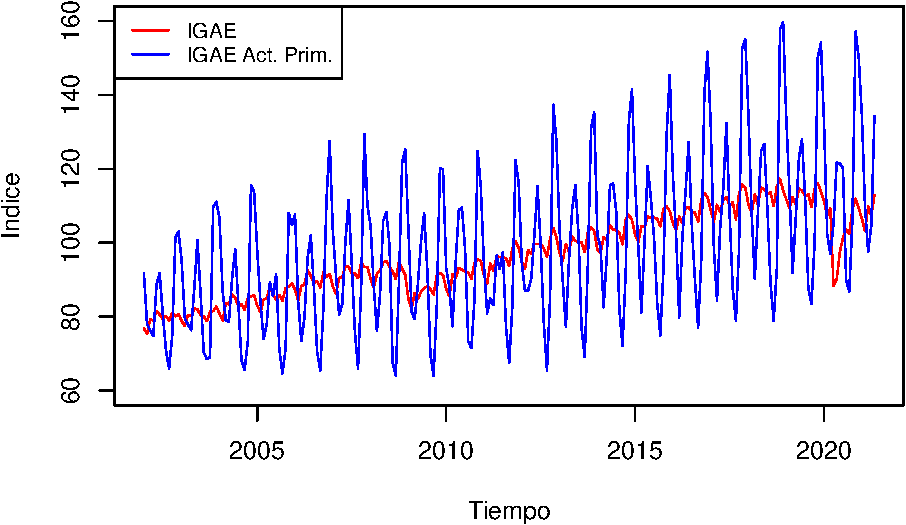
\includegraphics{index_files/figure-latex/fig1-1} 

}

\caption{Indicador Global de Actividad Económica (IGAE) Global y para las Actividades Primarias (2008=100), Ene.2002 - May.2021}\label{fig:fig1}
\end{figure}

Como se puede observar, el IGAE del total de la economía muestra, principalmente, que el enfoque del tiempo es más relevante. Es decir, que existe cierta persistencia en el indicador, lo que significa que la economía crece en razón del crecimiento reportado en periodos pasados. No obstante, lo que no podemos reconocer es que los eventos futuros tienen un efecto en el desempeño de la economía hoy día. Así, no es común observar cambios abruptos
del indicador, salvo por la crisis global de 2008 y la reciente crisis causada
por la Covid-19.

\begin{figure}

{\centering 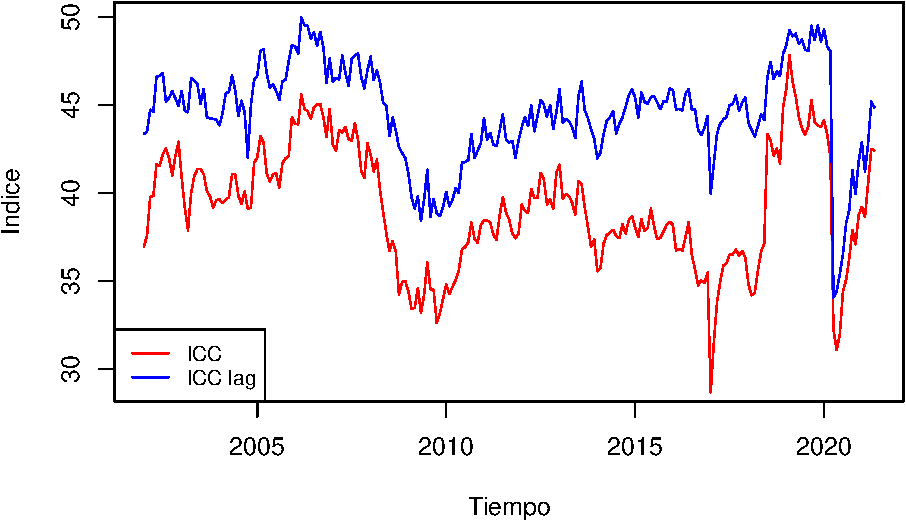
\includegraphics{index_files/figure-latex/fig2-1} 

}

\caption{Índice de Confianza del Consumidor (ICC): General y resultado de ¿Cómo considera usted la situación economica del país hoy en día comparada con la de hace 12 meses? (puntos), Ene.2002-may.2021}\label{fig:fig2}
\end{figure}

Por el contrario, el IGAE de las actividades primarias muestra una presencia
significativa de la importancia de la frecuencia. No pasa desapercibido que
existen muchos ciclos en la evolución del indicador. Algo que suena común
en las actividades primarias, cuya producción depende de eventos que son
ciclícos agrícolas asociados con el clima u otros factores determinantes de la
oferta de productos agrícolas. Otro factor que puede incluir en el indicador
son elementos de demanda, más que los de oferta. Por ejemplo, el consumo
de alimentos típicos de algunas temporadas del año.

Como segundo ejemplo, en la Figura \ref{fig:fig2} se ilustra la evolución reciente del índice de Confianza del Consumidor (ICC) en dos de sus versiones: i) el Índice global y ii) el Índice de confianza de los consumidores cuando estos consideran la situación actual en la economía en relación el año anterior.

Destacamos que el ICC mide las expectativas de los consumidores en
razón de la información pasada y de la esperada, segun dichos consumidores.

\begin{figure}

{\centering 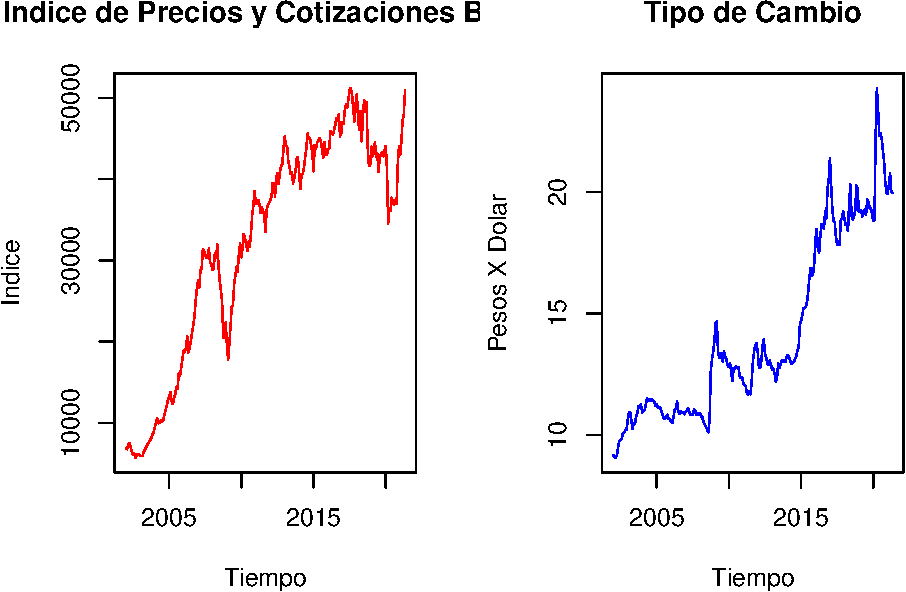
\includegraphics{index_files/figure-latex/fig3-1} 

}

\caption{índice de Precios y Cotizaciones de la Bolsa Mexicana de Valores (Panel Derecho) y Tipo de Cambio para Solventar Obligaciones en Moneda Extranjera, pesos por dólar (Panel izquierdo), Ene.2002-May.2021 }\label{fig:fig3}
\end{figure}

Así, es probable que las dos series de tiempo exhiban un gran peso para los
eventos pasados, pero a la vez, un componente -probablemente menor- del
componente de frecuencia. Esto último en razón de que los consumidores
suelen considerar en sus expectativas de consumo los periódos cíclicos de la
economía: temporadas navideñaas, pagos de colegiaturas, etc. Este sengundo
ejemplo tambien ilustra que la confianza del consumidor no necesariamente
está directamente correlacionada con el desempeño de la economía.

Como tercer ejemplo se muestra la evolución de dos series. La Figura \ref{fig:fig3} ilustra el comportamiento reciente de dos indicadores que son referencia para los inversionistas. Por un lado, se ubica el índice de Precios y Cotizaciones de la BMV (IPC), el cuál refleja el valor de las acciones de empresas que cotizan en la BMV y el volumen de acciones comercializadas, en conjunto. De esta forma, se ha interpretado que el IPC refleja el rendimiento del capital promedio invertido en las empresas que cotizan en la BMV.

Por otro lado, en la Figura \ref{fig:fig3} se presenta la evolución del Tipo de Cambio (TDC)\{indicador financiero que se suele utilizar como medio de reserva de valor. Esto, en razón de que el TDC es conocido como un instrumento que en momentos de crisis toma valores contraciclicos de la economía mexicana. No obstante, ambos indicadores no son comparables. Para hacerlos comparbles
en la Figura \ref{fig:fig4} se presentan en versión índice con una base en el primer mes de la muestra.

\begin{figure}

{\centering 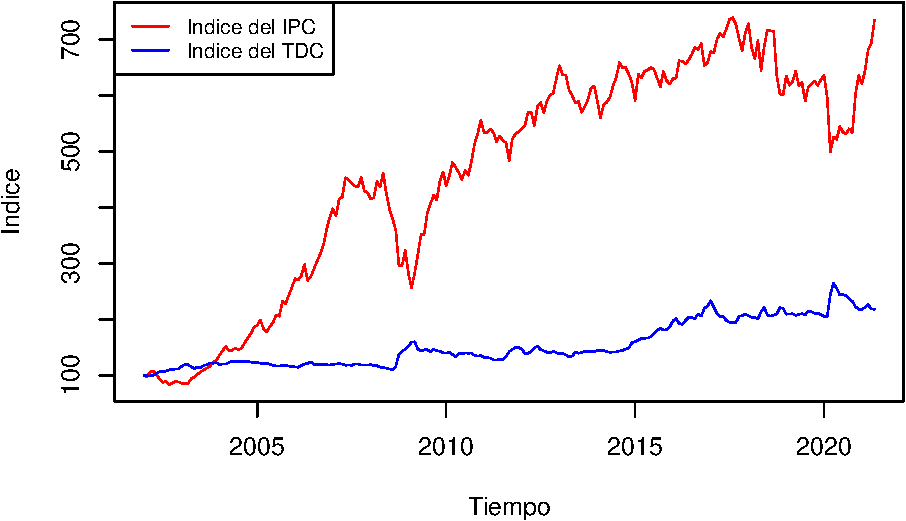
\includegraphics{index_files/figure-latex/fig4-1} 

}

\caption{Índice del índice de Precios y Cotizaciones de la Bolsa Mexicana de Valores (Panel Derecho) e Índice del Tipo de Cambio para Solventar Obligaciones en Moneda Extranjera (ambos enero de 2002 = 100), pesos por dólar (Panel izquierdo), Ene.2002-May.2021 }\label{fig:fig4}
\end{figure}

En la perspectiva de la Figura \ref{fig:fig4} se puede apreciar que el TDC no es tan rentable, ya que una inversión en la BMV mediante el IPC, en el largo plazo, muestra más redimientos. Asimismo, la Figura \ref{fig:fig4} ilustra que en ambas series se observa un dominio de la condición de tiempo y no uno de frecuencia. Es decir, tanto el IPC como el TDC no responden a condiciones como ciclos o temporadas que si son observables en actividades económicas como las
primarias.

Finalmente, la Figura \ref{fig:fig5} ilustra un característica que también resulta de gran interés en el analásis de series de tiempo: los datos de alta frecuencia y de comportamiento no regular. Como se puede observar, en la Figura \ref{fig:fig5} se muestran las diferencias logarítmicas de las series de IGAE de la actividad total, el IPC y el TDC.

\begin{figure}

{\centering 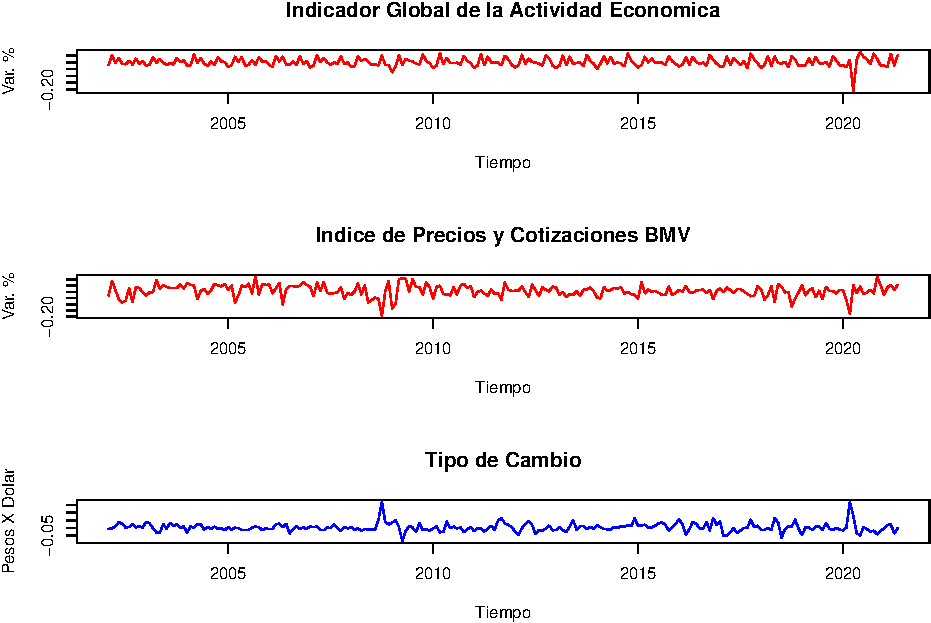
\includegraphics{index_files/figure-latex/fig5-1} 

}

\caption{Tasas de Crecimiento mensuales (diferencias logarítmicas) de Indicador Global de la Actividad Económica, Índice de Precios y Cotizaciones de la Bolsa Mexicana de Valores (Panel Derecho) y Tipo de Cambio para Solventar Obligaciones en Moneda Extranjera, Ene.2002-May.2021 }\label{fig:fig5}
\end{figure}

Dichas diferencia se pueden interpretar como una tasa de crecimiento de las series por las siguientes razones. Consideremos una serie de tiempo dada por \(y_t\), cuya versión logarítmica es \(ln(y_t\)). De esta forma, la diferencia logarítmica esta dada por la ecuación \eqref{eq:difflog}:

\begin{equation}
   \Delta ln(y_t) = ln(y_t) - ln(y_{t-1}) = ln \left( \frac{y_t}{y_{t-1}} \right)
   \label{eq:difflog}
\end{equation}

Ahora bien, si retomamos la definición de tasa de crecimiento (TC) de una serie de tiempo \(y_t\) entre el periodo \(t\) y \(t-1\) podemos obtener que:

\begin{equation}
    TC = \frac{y_t - y_{t-1}}{y_{t-1}} = \frac{y_t}{y_{t-1}} - 1
    \label{eq:TC}
\end{equation}

De esta forma, si tomamos el logarítmo de la expresión de la ecuación \eqref{eq:TC} obtenemos la siguiente aproximación:

\begin{equation}
    \frac{y_t}{y_{t-1}} -1  \approx ln \left( \frac{y_t}{y_{t-1}} \right) = ln(y_t) - ln(y_{t-1})
    \label{eq:TCDiffLog}
\end{equation}

La ecuación \eqref{eq:TCDiffLog} es cierta cuando los valores de \(y_t\) y \(y_{t-1}\) son muy parecidos, es decir, cuando las variaciones no son tan abruptas. Otra forma de interpretar la ecuación \eqref{eq:TCDiffLog} es que para tasas de crecimiento pequeñas, se puede utilizar como una buena aproximación a la diferencia logarítmica mostrada en la ecuación \eqref{eq:difflog}.

En la Figura \ref{fig:fig5} se reportan las diferencias logarítmicas del IGAE, IPC y TDC, todos, como una media de distitntos tipos de redimientos. Es decir, podemos decir que un capitalista promedio (suponiendo que solo puede invertir en la actividad económica, en la bolsa o en el dólar), puede observar que le es más redituable en función de sus preferencias.

Notése que la dinámica de las variaciones de cada una de las series es significativamente diferente. Destaca que el TDC es una de las variables que, en general, no muestra grandes cambios a lo largo del tiempo. No obstante, se han observado cambios radicales, cuando menos en el año 2008. Lo anterior, son caracteristicas que se han observado para el IPC. En cambio, el IGAE muestra un comportamiento más estable o estacionario.

\hypertarget{hello-bookdown}{%
\chapter{Hello bookdown}\label{hello-bookdown}}

All chapters start with a first-level heading followed by your chapter title, like the line above. There should be only one first-level heading (\texttt{\#}) per .Rmd file.

\hypertarget{a-section}{%
\section{A section}\label{a-section}}

All chapter sections start with a second-level (\texttt{\#\#}) or higher heading followed by your section title, like the sections above and below here. You can have as many as you want within a chapter.

\hypertarget{an-unnumbered-section}{%
\subsection*{An unnumbered section}\label{an-unnumbered-section}}
\addcontentsline{toc}{subsection}{An unnumbered section}

Chapters and sections are numbered by default. To un-number a heading, add a \texttt{\{.unnumbered\}} or the shorter \texttt{\{-\}} at the end of the heading, like in this section.

\hypertarget{cross}{%
\chapter{Cross-references}\label{cross}}

Cross-references make it easier for your readers to find and link to elements in your book.

\hypertarget{chapters-and-sub-chapters}{%
\section{Chapters and sub-chapters}\label{chapters-and-sub-chapters}}

There are two steps to cross-reference any heading:

\begin{enumerate}
\def\labelenumi{\arabic{enumi}.}
\tightlist
\item
  Label the heading: \texttt{\#\ Hello\ world\ \{\#nice-label\}}.

  \begin{itemize}
  \tightlist
  \item
    Leave the label off if you like the automated heading generated based on your heading title: for example, \texttt{\#\ Hello\ world} = \texttt{\#\ Hello\ world\ \{\#hello-world\}}.
  \item
    To label an un-numbered heading, use: \texttt{\#\ Hello\ world\ \{-\#nice-label\}} or \texttt{\{\#\ Hello\ world\ .unnumbered\}}.
  \end{itemize}
\item
  Next, reference the labeled heading anywhere in the text using \texttt{\textbackslash{}@ref(nice-label)}; for example, please see Chapter \ref{cross}.

  \begin{itemize}
  \tightlist
  \item
    If you prefer text as the link instead of a numbered reference use: \protect\hyperlink{cross}{any text you want can go here}.
  \end{itemize}
\end{enumerate}

\hypertarget{captioned-figures-and-tables}{%
\section{Captioned figures and tables}\label{captioned-figures-and-tables}}

Figures and tables \emph{with captions} can also be cross-referenced from elsewhere in your book using \texttt{\textbackslash{}@ref(fig:chunk-label)} and \texttt{\textbackslash{}@ref(tab:chunk-label)}, respectively.

See Figure \ref{fig:nice-fig}.

\begin{Shaded}
\begin{Highlighting}[]
\FunctionTok{par}\NormalTok{(}\AttributeTok{mar =} \FunctionTok{c}\NormalTok{(}\DecValTok{4}\NormalTok{, }\DecValTok{4}\NormalTok{, .}\DecValTok{1}\NormalTok{, .}\DecValTok{1}\NormalTok{))}
\FunctionTok{plot}\NormalTok{(pressure, }\AttributeTok{type =} \StringTok{\textquotesingle{}b\textquotesingle{}}\NormalTok{, }\AttributeTok{pch =} \DecValTok{19}\NormalTok{)}
\end{Highlighting}
\end{Shaded}

\begin{figure}

{\centering 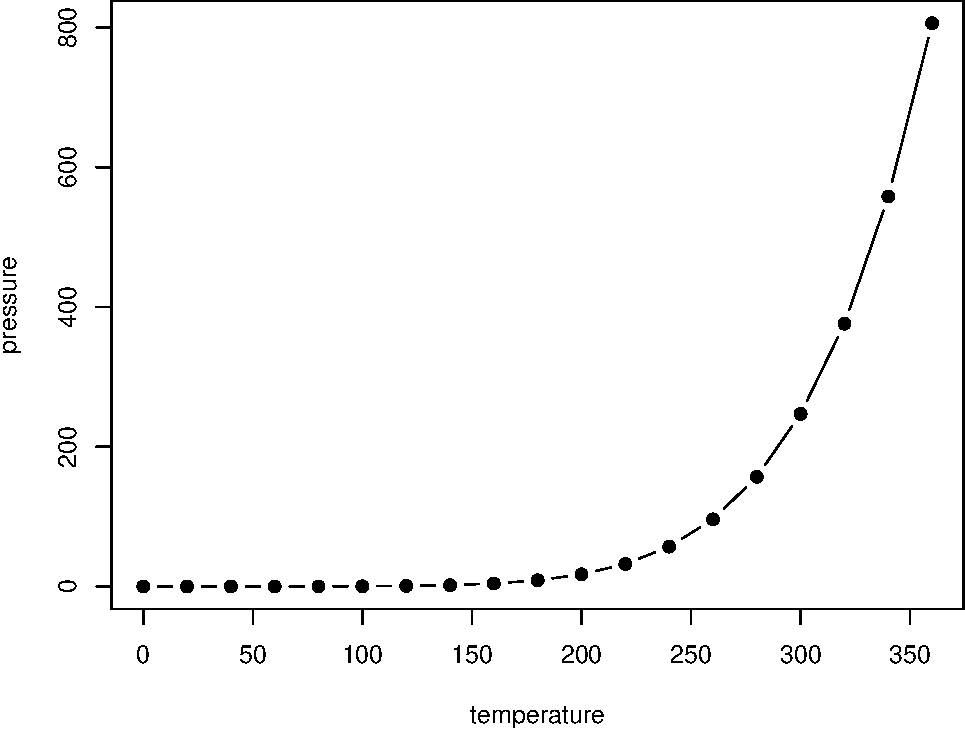
\includegraphics[width=0.8\linewidth]{02-cross-refs_files/figure-latex/nice-fig-1} 

}

\caption{Here is a nice figure!}\label{fig:nice-fig}
\end{figure}

Don't miss Table \ref{tab:nice-tab}.

\begin{Shaded}
\begin{Highlighting}[]
\NormalTok{knitr}\SpecialCharTok{::}\FunctionTok{kable}\NormalTok{(}
  \FunctionTok{head}\NormalTok{(pressure, }\DecValTok{10}\NormalTok{), }\AttributeTok{caption =} \StringTok{\textquotesingle{}Here is a nice table!\textquotesingle{}}\NormalTok{,}
  \AttributeTok{booktabs =} \ConstantTok{TRUE}
\NormalTok{)}
\end{Highlighting}
\end{Shaded}

\begin{table}

\caption{\label{tab:nice-tab}Here is a nice table!}
\centering
\begin{tabular}[t]{rr}
\toprule
temperature & pressure\\
\midrule
0 & 0.0002\\
20 & 0.0012\\
40 & 0.0060\\
60 & 0.0300\\
80 & 0.0900\\
\addlinespace
100 & 0.2700\\
120 & 0.7500\\
140 & 1.8500\\
160 & 4.2000\\
180 & 8.8000\\
\bottomrule
\end{tabular}
\end{table}

\hypertarget{parts}{%
\chapter{Parts}\label{parts}}

You can add parts to organize one or more book chapters together. Parts can be inserted at the top of an .Rmd file, before the first-level chapter heading in that same file.

Add a numbered part: \texttt{\#\ (PART)\ Act\ one\ \{-\}} (followed by \texttt{\#\ A\ chapter})

Add an unnumbered part: \texttt{\#\ (PART\textbackslash{}*)\ Act\ one\ \{-\}} (followed by \texttt{\#\ A\ chapter})

Add an appendix as a special kind of un-numbered part: \texttt{\#\ (APPENDIX)\ Other\ stuff\ \{-\}} (followed by \texttt{\#\ A\ chapter}). Chapters in an appendix are prepended with letters instead of numbers.

\hypertarget{footnotes-and-citations}{%
\chapter{Footnotes and citations}\label{footnotes-and-citations}}

\hypertarget{footnotes}{%
\section{Footnotes}\label{footnotes}}

Footnotes are put inside the square brackets after a caret \texttt{\^{}{[}{]}}. Like this one \footnote{This is a footnote.}.

\hypertarget{citations}{%
\section{Citations}\label{citations}}

Reference items in your bibliography file(s) using \texttt{@key}.

For example, we are using the \textbf{bookdown} package \citep{R-bookdown} (check out the last code chunk in index.Rmd to see how this citation key was added) in this sample book, which was built on top of R Markdown and \textbf{knitr} \citep{xie2015} (this citation was added manually in an external file book.bib).
Note that the \texttt{.bib} files need to be listed in the index.Rmd with the YAML \texttt{bibliography} key.

The \texttt{bs4\_book} theme makes footnotes appear inline when you click on them. In this example book, we added \texttt{csl:\ chicago-fullnote-bibliography.csl} to the \texttt{index.Rmd} YAML, and include the \texttt{.csl} file. To download a new style, we recommend: \url{https://www.zotero.org/styles/}

The RStudio Visual Markdown Editor can also make it easier to insert citations: \url{https://rstudio.github.io/visual-markdown-editing/\#/citations}

\hypertarget{pene}{%
\chapter{pene}\label{pene}}

\hypertarget{ecuaciones}{%
\section{ecuaciones}\label{ecuaciones}}

Here is an equation.

\begin{equation} 
  f\left(k\right) = \binom{n}{k} p^k\left(1-p\right)^{n-k}
  \label{eq:binom}
\end{equation}

You may refer to using \texttt{\textbackslash{}@ref(eq:binom)}, like see Equation \eqref{eq:binom}.

\hypertarget{theorems-and-proofs}{%
\section{Theorems and proofs}\label{theorems-and-proofs}}

Labeled theorems can be referenced in text using \texttt{\textbackslash{}@ref(thm:tri)}, for example, check out this smart theorem \ref{thm:tri}.

\begin{theorem}
\protect\hypertarget{thm:tri}{}\label{thm:tri}For a right triangle, if \(c\) denotes the \emph{length} of the hypotenuse
and \(a\) and \(b\) denote the lengths of the \textbf{other} two sides, we have
\[a^2 + b^2 = c^2\]
\end{theorem}

Read more here \url{https://bookdown.org/yihui/bookdown/markdown-extensions-by-bookdown.html}.

\hypertarget{callout-blocks}{%
\section{Callout blocks}\label{callout-blocks}}

The \texttt{bs4\_book} theme also includes special callout blocks, like this \texttt{.rmdnote}.

You can use \textbf{markdown} inside a block.

\begin{Shaded}
\begin{Highlighting}[]
\FunctionTok{head}\NormalTok{(beaver1, }\AttributeTok{n =} \DecValTok{5}\NormalTok{)}
\CommentTok{\#\textgreater{}   day time  temp activ}
\CommentTok{\#\textgreater{} 1 346  840 36.33     0}
\CommentTok{\#\textgreater{} 2 346  850 36.34     0}
\CommentTok{\#\textgreater{} 3 346  900 36.35     0}
\CommentTok{\#\textgreater{} 4 346  910 36.42     0}
\CommentTok{\#\textgreater{} 5 346  920 36.55     0}
\end{Highlighting}
\end{Shaded}

It is up to the user to define the appearance of these blocks for LaTeX output.

You may also use: \texttt{.rmdcaution}, \texttt{.rmdimportant}, \texttt{.rmdtip}, or \texttt{.rmdwarning} as the block name.

The R Markdown Cookbook provides more help on how to use custom blocks to design your own callouts: \url{https://bookdown.org/yihui/rmarkdown-cookbook/custom-blocks.html}

\hypertarget{sharing-your-book}{%
\chapter{Sharing your book}\label{sharing-your-book}}

\hypertarget{publishing}{%
\section{Publishing}\label{publishing}}

HTML books can be published online, see: \url{https://bookdown.org/yihui/bookdown/publishing.html}

\hypertarget{pages}{%
\section{404 pages}\label{pages}}

By default, users will be directed to a 404 page if they try to access a webpage that cannot be found. If you'd like to customize your 404 page instead of using the default, you may add either a \texttt{\_404.Rmd} or \texttt{\_404.md} file to your project root and use code and/or Markdown syntax.

\hypertarget{metadata-for-sharing}{%
\section{Metadata for sharing}\label{metadata-for-sharing}}

Bookdown HTML books will provide HTML metadata for social sharing on platforms like Twitter, Facebook, and LinkedIn, using information you provide in the \texttt{index.Rmd} YAML. To setup, set the \texttt{url} for your book and the path to your \texttt{cover-image} file. Your book's \texttt{title} and \texttt{description} are also used.

This \texttt{bs4\_book} provides enhanced metadata for social sharing, so that each chapter shared will have a unique description, auto-generated based on the content.

Specify your book's source repository on GitHub as the \texttt{repo} in the \texttt{\_output.yml} file, which allows users to view each chapter's source file or suggest an edit. Read more about the features of this output format here:

\url{https://pkgs.rstudio.com/bookdown/reference/bs4_book.html}

Or use:

\begin{Shaded}
\begin{Highlighting}[]
\NormalTok{?bookdown}\SpecialCharTok{::}\NormalTok{bs4\_book}
\end{Highlighting}
\end{Shaded}


  \bibliography{book.bib,packages.bib}

\end{document}
